\chapter{Modelado de la Solución}
Como se mencionó en el capítulo anterior, el problema principal surge de la no utilización
de métodos que permitan validar los documentos digitales, emitidos por la Secretaría de Extensión de la \glsfirst{fce} de la \glsfirst{unam}.
En este capítulo se explica cómo abordar la solución a este problema.


Se propone un sistema que permita al usuario consultar la validez  de sus documentos digitales   por la entidad que los emitió
  y cuando se publicó, asimismo que permita a los gestores de la organizaciones subir  nuevos documentos o algún identificador  para comprobar
de manera inequívoca si fue emitido por ellos, aun cómo mostrar datos relacionados al evento de la institución u organización.
Con esta propuesta de sistema, se atenderían los aspectos mencionados en cuanto a las necesidades de brindar un medio por el cual
se pueda verificar que la documentación de las actividades desarrolladas por la  
Secretaría de Extensión de la \gls{fce} no fue adulterada, modificada o cambiada.


En cuestiones generales para solucionar los problemas se propone realizar un sistema que permita a la 
Secretaría de Extensión de la \gls{fce} de la \gls{unam} :

\begin{enumerate}
    \item Dar validez a un documento por tiempo determinado y gestionar sus estados.
    \item Definir qué entidades externas puedan validar la integridad de documentos digitales emitido por la Universidad.
    \item Permitir acceso a todo público al sistema para la validación.
    \item Proteger la privacidad de los datos que pertenecen a los documentos.
\end{enumerate}

A tales efectos los ítems recientemente expuestos se pueden lograr con la utilización de la tecnología Blockchain, 
otorgando inmutabilidad a los datos almacenados y que ellos sean accesibles a todo público.
En cuanto a protección de la privacidad es necesario utilizar, algún método criptográfico 
para que los datos sean leídos,  solo por las partes autorizadas.
Y por último, para que las entidades o cualquier individuo pueda validar el documento digital, si es el mismo
que emitió la Secretaría de Extensión de la \gls{fce}. 

\section{Procesos para la Construcción del Sistema}
Serán necesarios para el diseño, modelado y desarrollo de la solución definir las herramientas a utilizar,
y los pasos.
\begin{enumerate}
    \item Definición de métodos y tecnologías a utilizar.
    \item Diseño de la solución.
    \item Desarrollo del diseño propuesto.
    \item Ensayos y validaciones del funcionamiento.
\end{enumerate}


\subsection{ Análisis de Tecnologías y Métodos para Validaciones}
Para poder realizar la propuesta de sistema, hay que determinar métodos y tecnologías  necesarias para llevarla a cabo.
Existen distintos tipos de métodos para validar los certificados con la  Blockchain como el estándar BlockCerts, OpenCerts y la \gls{bfa}.

% BlockCerts es un estándar abierto  que permite  almacenar y verificar documentos en la Blockchain,
% generar el hash a partir de un certificado o documento y  almacenarla en una transacción de la red de Bitcoin o Etherum u otra Blockchain.
% El estándar es muy útil y cuenta con una aplicación movil para poder verificar los documentos digitales, 
% donde los usuarios pueden obtener una cuenta propia. Su funcionamiento está descrito en el propio sitio web.

% \begin{figure}[H]
%   \centering
%   {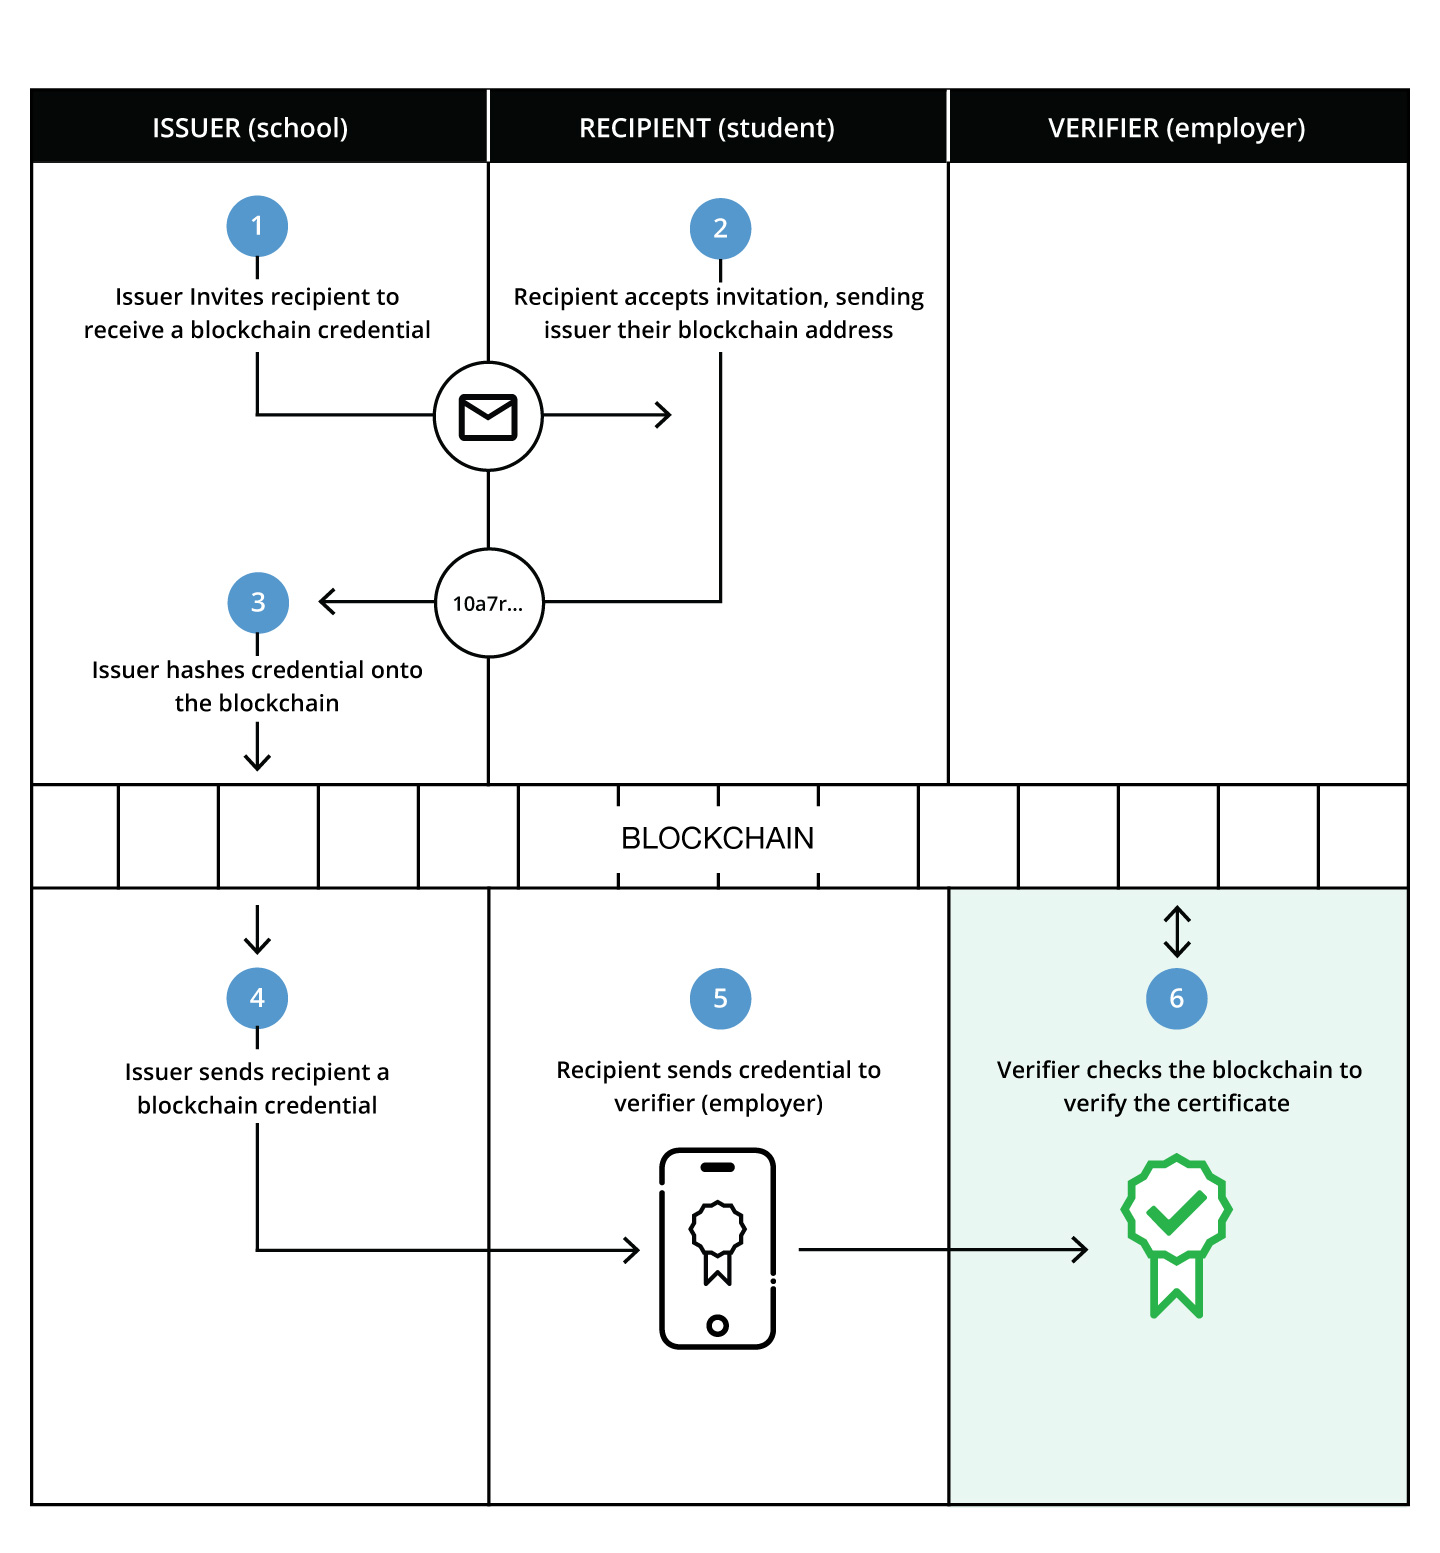
\includegraphics[scale=0.3]{blockcerts_how_it_works.jpg}}
%   \caption{Imagen extraída de la página oficial de BlockCerts}
%   \label{img:blockcerts_how_it_works}
% \end{figure}

% Este es el flujo básico que también se 
% puede visualizar en  la figura \ref{img:blockcerts_how_it_works}   para comprobar que
% un certificado se encuentra almacenado en la  Blockchain y es validado por un instituto.

% En el paso 1, el emisor o institución invita a un usuario a que brinde su dirección de cuenta o su clave pública creada 
% descargando, la aplicación movil que provee BlockCerts. En el paso 2, el usuario envía al emisor su clave pública.
% El paso 3 y 4, el emisor crea el hash a partir del certificado y lo almacena en la  Blockchain para luego enviar un archivo de tipo json \footnote{JavaScript Object Notation es un formato basado en texto estándar para representar datos estructurados \cite[]{mozilla_trabajando_json}.}, que contiene
% la información sobre el documento al estudiante o dueño del certificado. En el paso 5, puede enviar este documento a cualquier empresa o individuo que dese.
%  En el paso 6 el usuario que contiene el archivo puede verificarlo en el sitio web de  BlockCerts \cite[]{blockcerts_introduction_nodate}. 

% Este estándar es muy completo y permite a los usuarios gestionar sus propios certificados, pero lo que se busca en la investigación, 
% es desarrollar una propuesta de sistema donde un usuario puede abstraer el concepto de  Blockchain sin controlar una cuenta, enfoncadonce solamente en mantener guardados
% sus certificados.


% Otra sistema es OpenCerts que funciona generando 
% un código único a partir del certificado e información extra considerada como necesaria para validar el documento en el futuro, y luego se crea un archivo con extensión  “.opencerts ”;
% Dicho archivo se al sitio web de OpenCerts y compara el contenido con el almacenado en la  Blockchain para verificar si a existido el certificado en cuestión.
% Para dar de alta los certificados usa smart contract donde también crean los métodos para emitir o revocar un documento.

% \begin{figure}[H]
%   \centering
%   {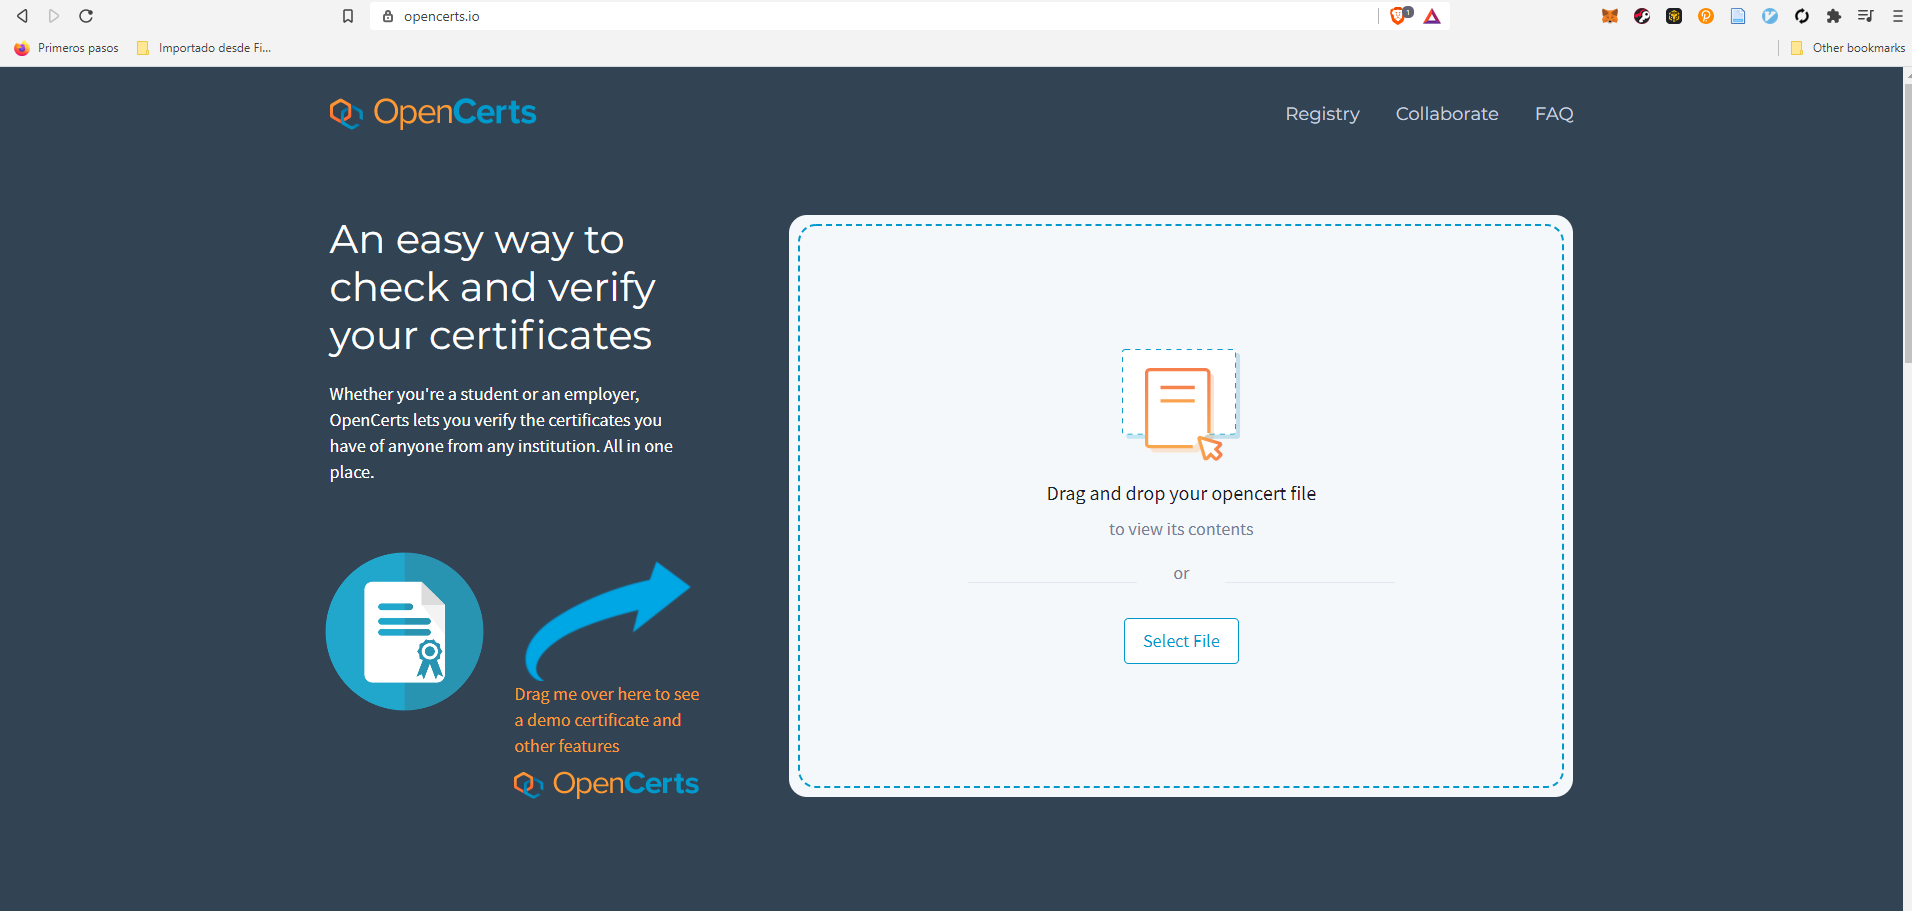
\includegraphics[scale=0.3]{OpenCerts_Home.png}}
%   \caption{página Web de OpenCerts}
%   \label{img:opencerts_home}
% \end{figure}

% En la imagen \ref{img:opencerts_home} se puede observar lo sencillo que es verificar un documento. Simplemente se arrastra el  archivo de extensión“.opencerts”
% y se buscará en la  Blockchain si realmente fue emitido por alguna entidad.
% OpenCerts utiliza los smart contract en la  Blockchain de Etherum. También utiliza tecnologías como Ract.js, Metamask, Web3.js, entre otros. Lo que permite desarrollar
% un sistema de certificados totalmente descentralizados \cite[]{opencerts_gestion_nodate}. 


 La \gls{bfa}, la cual es una  Blockchain que utiliza el protocolo de consenso llamado  prueba de autoridad. El sitio web cuenta con una herramienta llamada sello de tiempo 2.0, que permite verificar cuándo se  selló un archivo y en qué bloque,
permite confirmar que (desde esa fecha) el archivo en cuestión no sufrió modificaciones. Utiliza el mismo método que las anteriores tecnologías, 
crear un hash a partir de un archivo y almacenar el hash en la Blockchain \cite[]{Blockchain_federal_argentina_bfa_2020}.

Estas tecnologías, permiten demostrar que una secuencia de bits o cualquier tipo de archivo (puede ser
 un documento o certificado) se mantuvo inalterable a partir del día que se almacenó su hash en la Blockchain o identificador único. Algunas de ellas 
cuentan con un flujo y trabajo más elaborado, pero al fin todas cumplen con el objetivo de asegurar a los interesados si existió algún cambio en datos
del documento o archivo en cuestión. 
Luego de analizar el funcionamiento de éstas, se pretende realizar una propuesta de sistema, que permita a una institución principalmente 
a la \gls{fce} emitir sus certificados validados y los participantes de los eventos  demostrar que sus 
 documentos digitales son totalmente auténticos y correspondiente  a su persona \cite[]{opencerts_gestion_nodate,blockcerts_faq_nodate,Blockchain_federal_argentina_bfa_2020}. 

\subsection{ Análisis de Tecnologías para Desarrollar en Blockchain}

Existen diferentes tecnologías para elaborar un sistema que necesita comunicarse con una red de peer to peer y leer o escribir en la Blockchain.
Primero hay que definir cómo se almacenará la información en la Blockchain, si hacerlo en una transacción de cualquier  Blockchain (como lo hace
BlockCerts) o realizar una lógica y almacenarla en una  Blockchain que soporte contratos inteligentes.
La ventaja de los smart contract es que permiten almacenar información específica como ser el nombre de una institución, sus participantes o
cualquier dato que se desee en una sola transacción o invocación a un método del smart contract ( mientras que el primer método se necesitará 
almacenar diferentes datos en diferentes transacciones, o realizar un hash que representará que un documento sigue inalterable).



Por conveniencia de esta investigación se almacenarán datos en los smart contact, permite obtener información directamente de 
la  Blockchain, como ser el nombre, áreas, eventos de la institución. Esta diferencia da lugar a la creación de aplicaciones, por la 
conveniencia de almacenar datos que pueden ser recuperados y leídos, permitirá tener seguridad par evitar cambios no autorizados y asegurar que la información este disponible,
, en comparación con el estándar de BlockCerts que permite hacer lo mismo, pero se necesita el archivo que almacena toda la información del emisor \cite[]{opencerts_gestion_nodate,blockcerts_introduction_nodate}.
A partir de este punto se enumeran las diferentes herramientas necesarias, para el desarrollo de un sistema de validación de certificados usando Blockchain.


Lo más importante es elegir la  Blockchain que se utilizará para las pruebas y desarrollo. Existen 
las  Blockchain locales y online, también Blockchains principales y de pruebas.
Están las  Blockchain de Ethereum, Binance Smart Chain, EOS, como redes principales y online; redes de pruebas como
Ropsten, Rinkeby, entre otros.  Una de las herramientas es Ganache \footnote{\url{https://www.trufflesuite.com/ganache}}, que permite
levantar una  Blockchain  local con configuraciones personalizadas.
La diferencia entre las  Blockchain serán los algoritmos de consenso propios de la red, la cantidad de nodos, pero 
para el desarrollo de la propuesta de sistema esas característica no son necesarias, mientras que la red se comporte similar a la de una red principal, la
cual estas últimas son más seguras.
Dependerá seleccionar la  Blockchain según las necesidades de la propuesta, si se utiliza los smart contract o otra manera \cite[]{truffle_suite_ganache_nodate}.

\subsubsection{Comunicación con Blockchain}
Es necesario un método o herramienta para comunicar las transacciones que se deben realizarse 
en la Blockchain, para ello se precisa de una wallet o billetera que permita enviar las transacciones 
y comunicarse con los smart contract, en este caso existen diferentes wallet, pero una de las usadas por desarrolladores
es Metamask, permite gestionar las cuentas de los usuarios de manera local, conectarse con diferentes Blockchain, 
recibir y enviar dinero e interactuar con los Smart Contract.
Se instala como una extensión del navegador en Google Chrome o Firefox,  es usado como puente entre una aplicación y la Blockchain \cite[]{dannen_introducing_2017,metamask_introduction_2021}. 
La herramienta se puede observar en la figura \ref{img:metamask_wallet}.
\begin{figure}[H]
  \centering
  {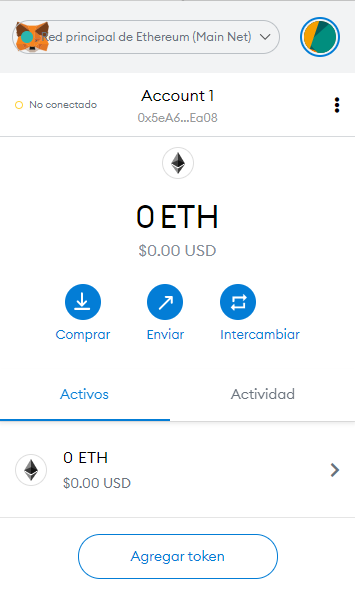
\includegraphics[scale=0.7]{MetaMask_Wallet.png}}
  \caption{MetaMask Plugin imagen extraída}
  \label{img:metamask_wallet}
\end{figure}
Por otro lado para la invocación de los métodos del contrato inteligente, se usa web3.js, que aporta las funcionalidades
necesarias para realizar las llamadas de procedimientos remotos a los nodos de la Blockchain, por la cual se pueden leer y escribir datos  abstrayendo la comunicación directamente 
y la creación de las transacciones, mientras la gestión de la cuenta de lo usuarios se realiza con MetaMask \cite[]{dannen_introducing_2017}.



\subsubsection{Programación en Blockchain}

Se deberá  decidir en qué  Blockchain se trabajará, porque los smart contract se escriben en un lenguaje específico,
en el caso de Etherum es Solidity, pero existen un gran número de  Blockchain que utilizan la misma estructura de Etherum para generar 
su propia  Blockchain con algunas diferencias, pero en cuanto al lenguaje de programación  para el desarrollo de los smart contract 
es el mismo. En este caso se utilizará Solidity porque existen documentaciones que describen su uso y es la más usada para el desarrollo de smart contract \cite[]{dannen_introducing_2017,ethereum_solidity_nodate}

\subsubsection{Publicación de Smart Contract}
Es necesario utilizar una herramienta  que permita enviar el código escrito con el lenguaje Solidity a la Blockchain, para 
ello existen herramientas tales como Remix o Truffle, las que permiten compilar y almacenar el smart contract en una red de prueba local como online.
En el caso de Remix es una herramienta que puede usarse de manera online o local. Permite desplegar el código en una  Blockchain de prueba local o 
de prueba online como Ropsten o una Mainnet como Etherum \cite[]{remix_deploy_nodate}.
 Truffle es un entorno de desarrollo, marco de pruebas y canalizados de activos para cadenas de bloques que utilizan la máquina virtual Ethereum (EVM), con el objetivo de facilitar el desarrollo
de proyectos con Blockchain, permite desplegar también de manera pública o privada, así mismo provee otras facilidades como gestión de paquetes,
automatización de pruebas, entre otras \cite[]{truffle_truffle_nodate}. 






\subsubsection{Desarrollo del font-end}
Se deben seleccionar las  herramientas que se necesitan para la creación de la interfaz de los usuarios 
que pretenden gestionar la información relacionada a la documentación digital y a la institución.
Al utilizar las tecnologías mencionadas, es necesario  un desarrollo web, donde se puede obtener  un servidor central o descentralizado
para almacenar datos de usuario, y conectando 
el front-end con la  Blockchain directamente. Esta última es conveniente para evitar manejar datos sensibles 
porque serían visibles a todo público, puede verificar la existencia de los datos y 
el servidor central no es necesario para la validación de documentos.
Para el desarrollo de un front-end es necesario la utilización de  tecnologías como  HTML, javascript y CSS o utilizar un framework como
ReactJS, VueJS o AngularJS, para desarrollar el sistema de manera organizada incluyendo todo lo requerido para la interfaz de usuario \cite[]{dannen_introducing_2017,educacionit_carrera_nodate}.

Para la creación de un sistema de validación de documentos digitales es conveniente utilizar los puntos importantes   del estándar BlockCert y  la utilización de los smart contract 
como lo hace OpenCert, también existen códigos fuentes que pueden ser reutilizados. Uno de ellos
son las herramientas que provee la  \gls{bfa}, por ejemplo la interfaz para que un usuario valide o selle un documento, este
código se encuentra escrito en VueJS, por lo que se optará
su uso para el desarrollo de la vista del usuario. Cabe aclarar que se puede realizar con cualquier otro framework (esto se puede
demostrar encontrando los diferentes proyectos existentes con diferentes tecnologías usadas o en cursos de desarrollo de  Blockchain con ReactJS 
% \footnote{\href{https://codeburst.io/build-a-cryptocurrency-dashboard-with-react-d9e476de91ef?gi=854fd33c74d7}{Ejemplo par Desarrolar con React}}.
o AngularJs \cite[]{Blockchain_federal_argentina_bfa_2020}. 
% \footnote{\href{https://medium.com/Blockchain-developer/learn-how-to-create-your-own-dapp-with-angular-part-i-688f24e0ad9e}{Ejemplo de como Desarrollar con Angular.}}).

\subsubsection{Criptografía}
La función hash es necesaria como parte de cualquier proyecto de documentos digitales visto, como lo usan BlockCert y OpenCert, también
las propias  Blockchain la usan para crear las direcciones de los bloques. Asimismo la \gls{bfa} usa esta función hash. 
Existen diferentes tipos como MD5, SHA y sus variaciones  por lo general en las Blockchains y 
en los sistemas o aplicaciones utilizan SHA-256, por su uso extendido  se elije esta última \cite[]{satoh_asic-hardware-focused_2007}.



\section{Análisis de la Propuesta de Sistema de Validación de Documentos Digitales}

Para que el sistema permita validar documentos digitales sin almacenar la información contenida en ella y 
evitar acceder a datos sensibles de un individuo, se utilizarán los métodos de los estándares o sistemas (BlockCerts y OpenCerts). En otras palabras, genera
un hash a partir de una secuencias de caracteres como valores de entrada y  se obtiene una salida de longitud fija, de este modo se  aumenta la dificultad
para conocer el contenido del documento y se genera un identificador único, el hash asegura que el documento no fue modificado y puede ser verificado usando nuevamente 
el mismo archivo original \cite[]{blockcerts_introduction_nodate,jirgensons_Blockchain_2018}.
Luego se necesitará información adicional, como ser el día en el cual el documento se creó, o si esta relacionado a algún evento de la organización que la emitió,
nombre de la organización, el nombre del Área o Departamento encargado de generar el documento y los datos extras que se necesiten. Por otro lado 
permitir a los encargados de emitir los certificados poder cambiar los estados de los documentos, por ejemplo, si pasado un tiempo un documento
ya no tiene validez, se puede cambiar el estado del documento a no válido, o darle una fecha de expiración si se necesitara.
Con esta información se creará   un smart contract que permita almacenar estos datos en la Blockchain, manteniéndolos inmutable 
a menos que se permita roles a usuarios específicos, con permisos para modificarlos.

\subsection{Bases del Sistema}\label{ss:basesistema}
La base del sistema es  mantener los documentos digitales o el hashes inalterables, para asegurar
que el contenido no cambió.

En primer lugar es gestionar los tipos de documentos que se manejan, definir cómo se almacenarán y asignarán  el/los
responsable/s de hacerlo, con la  posibilidad de cambiar algunas características de los documentos digitales \cite[]{opencerts_gestion_nodate}.
Por ejemplo, manejar estados de los documentos, que permita a los interesados de validar si el documento
fue emitido por la universidad o una institución. Los estados sirven para 
que el interesado pueda observar si la documentación venció o si está en algún estado específico.   
Los datos usados por los estándares como BlockCert y OpenCert son el hash del documento, que una vez almacenado
no se permite cambiarlo, cambiar estados, definir una fecha de creación y una fecha de expiración.

Los estándares  almacenan información relacionada con el lugar donde se emitió el documento \cite[]{opencerts_gestion_nodate}, esto se logra 
agregando información como el evento  que lanzó el certificado, por ejemplo, un cursado, un examen, etc, cualquier situación que pueda 
generar una documentación digital \cite[]{mit_media_lab_what_2016}.
El evento puede suceder en un lapso de tiempo o puede ser indeterminado, por ejemplo, 
un evento de un curso que su duración son 3 días, o un evento que inicia una fecha pero no se conoce cuando finalizará.

Los eventos suceden en algún sitio o área, al observar  la \glsfirst{fce} de la \glsfirst{unam} 
la Secretaría de Extensión es la encargada de realizar los eventos o actividades como cursos, o 
actividades externas, por ende, el  área encargada es la Secretaría de Extensión (A.L., comunicación personal, 02/10/2020).%\cite[]{larraburu_secretariextension_2020}.

Se podrá almacenar información como el nombre y las áreas de la institución, con  estos datos se obtiene qué área almacenó el documento digital, conocer el evento que 
se generó en una fecha determinada o indeterminada, si el documento puede caducar, y por último, 
si el documento fue generado por la institución, dando una validez de que existe en la Blockchain.

Estas informaciones, se obtuvieron de   relevamientos que explican  el funcionamiento de las aplicaciones para certificados digitales y las informaciones que son usadas
frecuentemente. Por  ejemplo, el estándar BlockCerts que almacena el hash del documento e información relacionada
al emisor \cite[]{blockcerts_faq_nodate}.

% \subsection{Diseño de la lógica}
% A continuación se muestra un diagrama de flujo de datos.

% \begin{figure}[hbt!]
%   \centering
%   {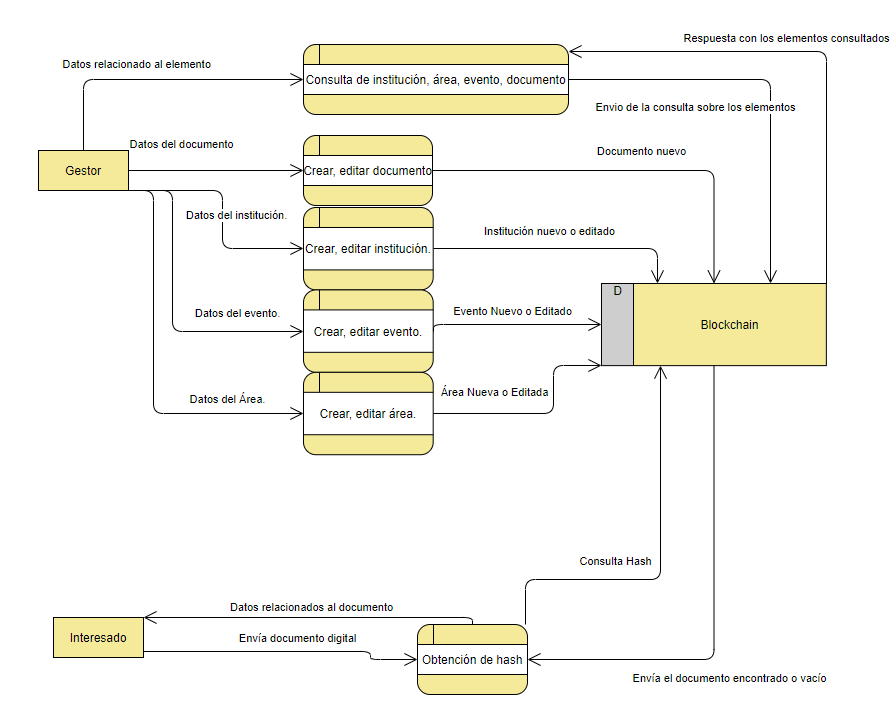
\includegraphics[scale=0.7]{Diagrama_Validacion_Documento.png}}
%   \caption{Diagrama de Flujos de datos, elaboración del Autor}
%   \label{img:flujo-datos}
% \end{figure}

% En la figura \ref{img:flujo-datos} se puede observar cómo fluyen los datos, el diagrama es una solución genérica sin entrar a los detalles.
% Pero el flujo de los datos serían principalmente almacenar los datos relacionados a un documento digital especifico. A partir de 
% uno o algunos responsables, ya que si cualquier individuo puede almacenar esta información, no tendría ninguna validez,
% por lo tanto solo los documentos almacenados mediante el uso del smart contract  serán válidos.

% Los interesados en el diagrama representan a cualquier individuo (como el propio dueño del documento digital, o una autoridad de la organización o persona externa de ella)
%, pudiendo obtener datos relacionado con el documento quién fue el emisor o si el documento fue realmente subido por la organización. 
% Pero para poder realizar tal verificación debe tener el documento digital en su posesión; de esta forma comprobar si 
% el contenido del documento no fue modificado y que fue emitido por la organización.

% Los gestores son los encargados de almacenar la información y serían personas que recae la responsabilidad
% de los documentos que se emiten.

\subsection{Solución Propuesta}
Para validar los documentos digitales de la Secretaría de Extensión de la \gls{fce} de la \gls{unam}, se propone crear un sistema,
basado en los protocolos definidos para la validación de documentos se utilizada tecnología Blockchain, 
para ello se realizará un smart contract que tendrá la lógica necesaria para almacenar datos relacionados
al documento, sin exponer datos sensibles de los intervinientes, y permite la validación del documento que permaneció sin cambios. 
También gestionar información de los documentos y cambiar estados futuros de ellos, almacenar 
el documento en la  Blockchain permite crear una relación única entre una cuenta y la información guardada,
habilita  seguir consultando los datos en el futuro. 

















 









